\documentclass[conference]{IEEEtran}
\IEEEoverridecommandlockouts
% The preceding line is only needed to identify funding in the first footnote. If that is unneeded, please comment it out.
\usepackage{cite}
\usepackage{amsmath,amssymb,amsfonts}
\usepackage{algorithmic}
\usepackage{graphicx}
\usepackage{textcomp}
\usepackage{xcolor}
\begin{document}

\title{\fontsize{20}{24}\selectfont Comparative Analysis of ResNet50 with Fully Connected Layers and YOLOv8 for Object Detection in Animal Detection Tasks}

\author{\IEEEauthorblockN{Nguyen Minh Nhut}
\IEEEauthorblockA{\textit{Student of Artificial Intelligence} \\
\textit{FPT University}\\
Ho Chi Minh City, Vietnam \\
minhnhut.ngnn@gmail.com}
\and
\IEEEauthorblockN{Truong Trong Nghia}
\IEEEauthorblockA{\textit{Student of Artificial Intelligence} \\
\textit{FPT University}\\
Ho Chi Minh City, Vietnam \\
email@example.com}
\and
\IEEEauthorblockN{Author Name}
\IEEEauthorblockA{\textit{Student of Artificial Intelligence} \\
\textit{University of ABC}\\
City, Country \\
email@example.com} \\
\and
\IEEEauthorblockN{Author Name}
\IEEEauthorblockA{\textit{Student of Artificial Intelligence} \\
\textit{University of ABC}\\
City, Country \\
email@example.com}\\
\and
\IEEEauthorblockN{Author Name}
\IEEEauthorblockA{\textit{Student of Artificial Intelligence} \\
\textit{University of ABC}\\
City, Country \\
email@example.com}
}
\maketitle
\begin{abstract}
Object detection in the context of animal detection tasks has become increasingly important for wildlife monitoring and conservation efforts. In this study, we conduct a comparative analysis between two prominent object detection frameworks: ResNet50 with fully connected layers and YOLOv8n (You Only Look Once). These frameworks are evaluated based on their performance, efficiency, and suitability for animal detection tasks. We explore their capabilities in accurately detecting and localizing animals in images and videos, considering factors such as detection speed, accuracy, and robustness to variations in environmental conditions. Through extensive experiments and evaluations on benchmark datasets, we aim to provide insights into the strengths and limitations of each framework, facilitating informed decision-making for researchers and practitioners in the field of wildlife monitoring and conservation.
\end{abstract}

\begin{IEEEkeywords}
Object Detection, ResNet50, YOLOv8n, Animal Detection.
\end{IEEEkeywords}

\section{Introduction}
Object detection algorithms have undergone significant advancements, primarily revolving around one-stage and two-stage approaches. Each method presents distinct advantages and drawbacks, thereby necessitating careful consideration based on the specific use case and performance criteria.

Two-stage algorithms, exemplified by faster R-CNN variants \cite{ren2015faster}, employ a region proposal network (RPN) to generate candidate object bounding boxes, refining predictions subsequently. These algorithms demonstrate superior accuracy, particularly in scenarios involving numerous object classes or cluttered scenes.

In contrast, one-stage algorithms like YOLO \cite{redmon2016you} and SSD \cite{liu2016ssd} predict object classes and bounding boxes in a single pass, resulting in expedited inference times and suitability for real-time applications. Nevertheless, these algorithms may exhibit lower accuracy when confronted with objects of varying scales and aspect ratios.

In this paper, we present a comparative analysis of two state-of-the-art object detection frameworks: ResNet50 with fully connected layers and YOLOv8, specifically tailored for animal detection tasks. We aim to investigate their performance, robustness, and suitability for real-world applications in wildlife monitoring scenarios. By conducting comprehensive experiments and evaluations on benchmark datasets, we seek to provide insights into the strengths and limitations of each approach, enabling practitioners to make informed decisions when choosing the most suitable method for their specific requirements.

\section{Related Work}

This section discusses various approaches employed for animal detection in videos and images. The prevalent approach in the domain of object detection, particularly in wild animal detection, is the utilization of Deep Learning models and Convolutional Neural Networks (CNNs). Many research papers have focused on the classification and localization of wild animals in images using Support Vector Machines. One such method was proposed by Michael J. Wilber and Walter J. Scheirer \cite{wilber2013animal}.

Archana et al. presented in their approach, an input video is divided into multiple frames, which then undergo a smoothing procedure \cite{archana2017artificial}. The subsequent steps involve the extraction of foreground animals through background subtraction from binary images. Morphological filtering is applied to further reduce noise from the extracted binary images. The process continues with cropping the extracted foreground animals using bounding boxes. Finally, the extracted foreground test image is compared with the training dataset using a backpropagation algorithm for recognition. Deep learning is the widely used approach for object detection.

A study conducted by Mahendra Kumar Gourisaria and Utkrisht Singh involved animal classification through the application of transfer learning models and CNNs \cite{gourisaria2022performance}. They trained these models on a dataset comprising over 28,000 animal images sourced from Google Images, encompassing 10 distinct animal classes. The models utilized in their research included VGG16 \cite{simonyan2014very}, EfficientNetB2 \cite{tan2019efficientnet}, ResNet101 \cite{he2016deep}, EfficientNetB7 \cite{tan2019efficientnet}, and ResNet50 \cite{he2016deep}.

Normaisharah Mamat and Mohd Fauzi Othman implemented the YOLOv5 model for animal detection \cite{mamat2022animal}. Stefan Schneider and Graham W. Taylor employed the YOLOv2 and RCNN models for animal detection \cite{schneider2018deep}. Their training dataset comprised images from the Reconyx Camera Trap and the self-labeled Gold Standard Snapshot Serengeti datasets. They achieved an accuracy exceeding 93.0(\%) and 76.7(\%) using the Fast RCNN model and 65.0(\%) and 43.3(\%) using YOLOv2 in the respective datasets.

Atri Saxena and Deepak Kumar Gupta utilized a dataset containing 31,774 images spanning 25 different classes \cite{saxena2021animal}. Their work involved the design of an object detection model based on SSD \cite{liu2016ssd} and Faster RCNN \cite{ren2015faster}. The results from their study indicated that the SSD model achieved 80.5(\%) mean Average Precision (mAP) at a detection speed of 100 frames per second, while the Faster R-CNN achieved 82.11(\%) mAP at a detection speed of 10 frames per second.

In a paper authored by Chunbiao Zhu and Thomas H. Li, a solution for low-quality cameras was proposed \cite{zhu2017towards}. They generated a flow map from the image and subsequently generated a Depth Map by utilizing the flow map and RGB information through the application of Simple Linear Iterative Clustering (SLIC). In this study, a CNN-based VGG model was employed. The original image, along with its depth map, was utilized as input to extract dual-channel perceptual deep features.

\section{Methodology}
\subsection{Dataset Description}
The dataset was compiled from diverse sources, including Kaggle datasets \cite{dave2023wild}. Initially, a substantial portion of our samples originated from the Animal Detection Images Dataset \cite{dave2023wild}, which is a labeled dataset.The resulting dataset comprises a total of 1304 images distributed as follows: 204 instances of Cheetah, 363 images of Tigers, 308 images of Lion, 212 images of Zebra, and 217 images of Leopards. In order to enhance our dataset for training purposes, we also added images from various sources, including unlabeled datasets and videos from platforms such as NatGeoWild and animal documentaries. To maintain a balanced and unbiased dataset, we meticulously divided it into training, testing, and validation sets. Each of these sets contains approximately an equal number of instances from each class. The dataset is also randomized, eliminating biases towards particular classes or features, thereby enhancing diversity in detection by the model. Figure \ref{fig:dataset_samples} shows the samples from the dataset. Table \ref{tab:distribution_samples} presents the distributions of samples of each category into the training set, validation set, and test set.

\begin{table}[htbp]
    \centering
    \caption{Distribution of samples in the dataset}
    \label{tab:distribution_samples}
    \begin{tabular}{cccc}
    \hline
    Category & Train Set & Test Set & Total\\
    \hline
    Lions & 200 & 108 & 308 \\
    Tigers & 329 & 34 & 363 \\
    Cheetah & 162 & 42 & 204 \\
    Leopards & 172 & 45 & 217 \\
    Zebra & 172 & 40 & 212 \\
    \hline
    Total & 1034 & 269 & 1304\\
    \hline
    \end{tabular}
\end{table}

\begin{figure}[htbp]
    \centering
    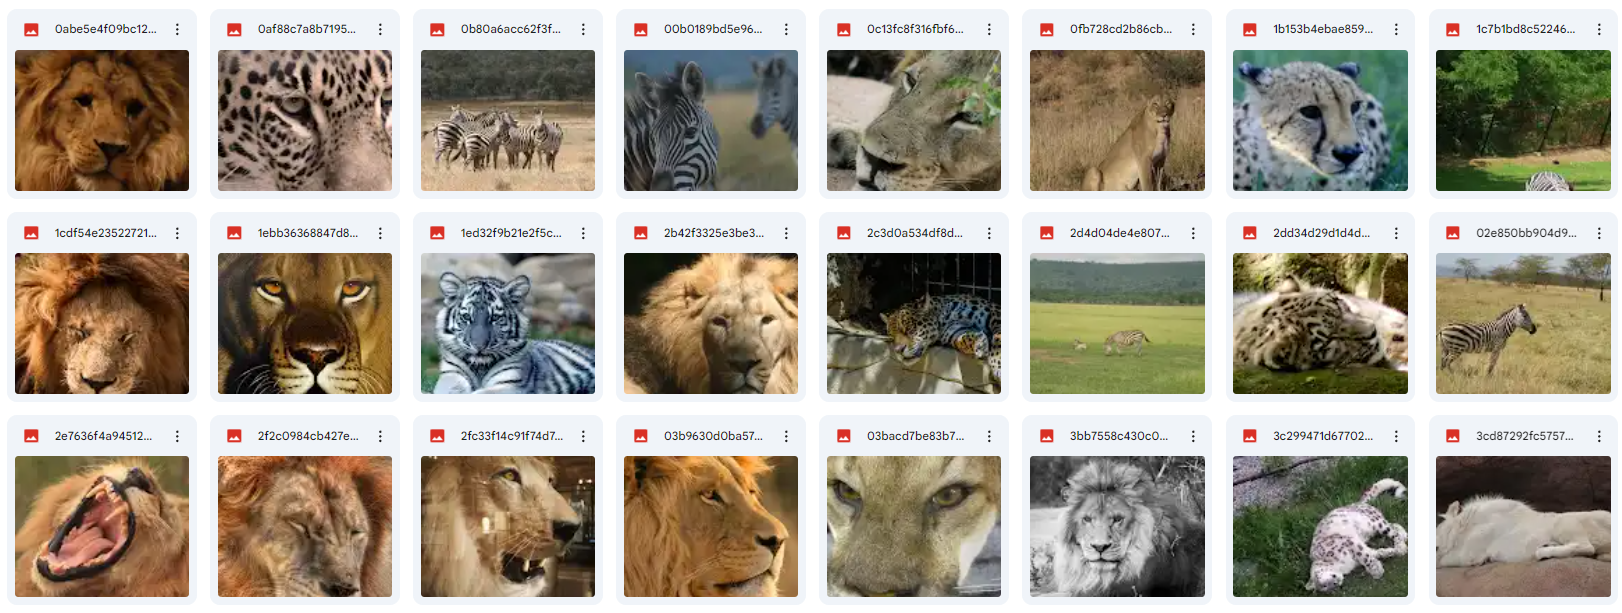
\includegraphics[width=3.4 in]{Dataset_pic.png}
    \caption{Samples from the dataset}
    \label{fig:dataset_samples}
\end{figure}

\subsection{Methodogy with YOLOv8}
\subsubsection{Preprocessing}

Figure \ref{fig:orginalDST} show the Original Dataset Structure. In summary, the dataset is already split into `train` and `test` subsets. Each subset contains N different classes like "Lion", "Tiger", "Zebra", etc. Each class has its own folder in the (train/test) subset that contains list of images and label text files. Labels are inside `Label` directory while the images are in the root of the class directory. 

Annotations are in format: "\{label\} \{x\_min\} \{y\_min\} \{x\_max\} \{y\_max\}" where coordinates are not normalized.

\begin{figure}[htbp]
    \centering
    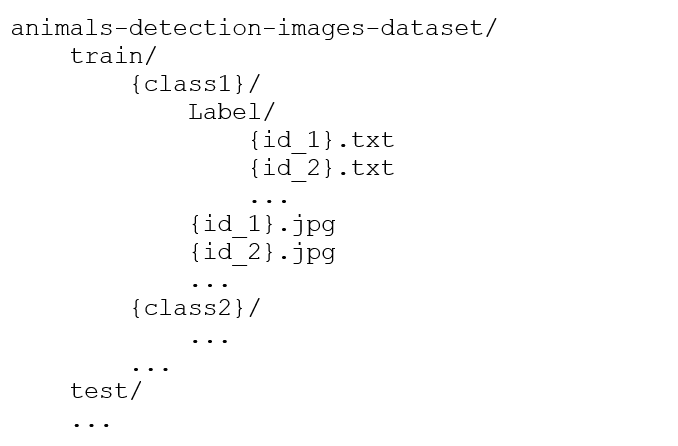
\includegraphics[width=3 in]{fig2.png}
    \caption{Original Dataset Structure }
    \label{fig:orginalDST}
\end{figure}
Dataset structure should be transformed to next format \ref{fig:YoloDST}.

\begin{figure}[htbp]
    \centering
    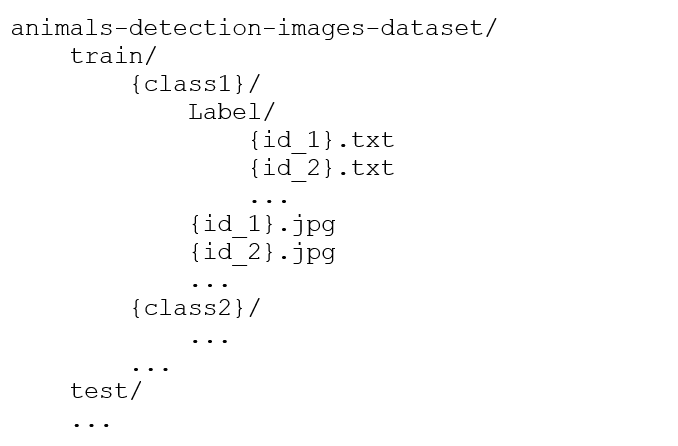
\includegraphics[width=3 in]{fig2.png}
    \caption{ Yolo Dataset Structure}
    \label{fig:YoloDST}
\end{figure}
Annotations should be in format: "\{label\_index\} \{x\_center\} \{y\_center\} \{width\} \{height\}" where coordinates are normalized.
\subsubsection{Architecture}
The YOLOv8 model architecture is utilized for wild animal object detection, as part of the YOLO (You Only Look Once) series of object detection models. Figure \ref{fig:Architecture of the wild animal detection model using Yolov8} illustrates the proposed architecture for wild animal detection using YOLOv8. YOLO was chosen due to its proven accuracy in real-time object detection tasks. YOLOv8 represents a state-of-the-art object detection model introduced by Ultralytics \cite{dave2023wild}. It is constructed on a hybrid backbone network, which combines the efficiency of convolutional neural networks with the power of spatial attention modules. Additionally, YOLOv8 introduces a novel anchor box design and loss function, enhancing detection performance for overlapping and small objects.

YOLOv8 is built with its Backbone as CSPDarknet53, which consists of 53 convolutional layers and is available in various sizes, including nano, small, medium, large, and extra-large. Considering the size of our dataset, we opted to train our model using the YOLOv8n architecture. YOLOv8n is specifically designed for faster inference and real-time applications compared to larger architectures like YOLOv8l and YOLOv8x. Its smaller size and reduced complexity make it more suitable for deployment on resource-constrained devices and scenarios where real-time processing is crucial, such as surveillance systems and autonomous vehicles. By utilizing YOLOv8n, we aim to achieve efficient and real-time wild animal detection without compromising accuracy.

\begin{figure}[htbp]
    \centering
    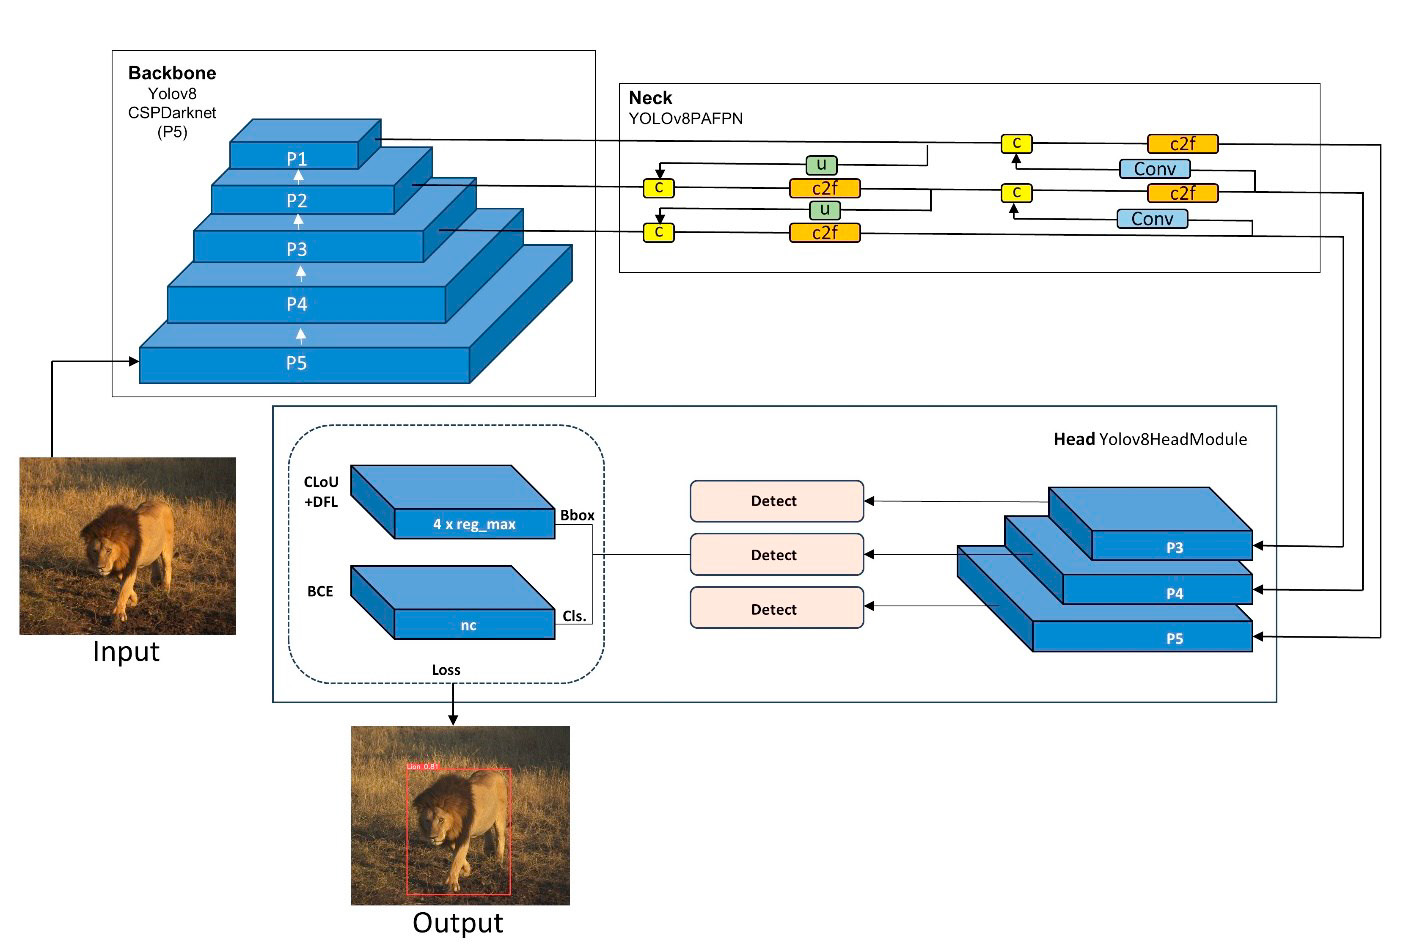
\includegraphics[width=3 in]{fig4.png}
    \caption{Architecture of the wild animal detection model using Yolov8}
    \label{fig:Architecture of the wild animal detection model using Yolov8}
\end{figure}

\subsection{Methodogy with ResNet50 Architecture}

\section{Experimental Results}
Your experimental results section goes here.

\section{Conclusion}
Your conclusion goes here.

\bibliographystyle{IEEEtran}
\bibliography{references}


\end{document}
